%use in documents with \subfile{tex/intro}
\documentclass[../../master.tex]{subfiles}

\begin{document}
	
\subsection{Secondary Structure Thermodynamics}
\label{sub:theory:thermodynamics}
% regardless of MFE or partition func
% this is the basis:
% assumption that thermodynamics define stability, i.e.
% gibbs free energy of a structure is stability (dill, tinoco1971)
% to compute energy efficiently, we need additivity (Dill)
% the general idea applies to crossing structures as well

The underlying idea of using thermodynamics for RNA secondary structure prediction is that of phrasing a notion of structural stability in terms of the Gibbs free energy change $\Delta G$ relative to the unfolded state containing no base pairs at all \parencite{tinoco_estimation_1971}:
\begin{equation}\label{eq:gibbs}
	\Delta G = \Delta H - T \Delta S \leq 0
\end{equation}
where $\Delta H$ is the (pressure- and volume-dependent) enthalpy change, $T$ the absolute temperature and $\Delta S$ the entropy change.

Furthermore, it is usually assumed that the free energy of a structure is the sum of its substructures' free energies \parencite{dill_additivity_1997}.
With this assumption, the computation of RNA structure free energies may be reduced to smaller subproblems but requires a well-defined model of secondary structure decomposition and energy assignment such as the nearest-neighbor model introduced in \autoref{ssub:theory:nnmodel}.



%\parencite{devoe_stability_1962}
%\parencite{tinoco_how_1999}



\subsubsection{The Nearest-Neighbor Energy Model}
\label{ssub:theory:nnmodel}

%For simplicity, only nested structures are considered here (see \autoref{sub:theory:pseudoknots}, \parencite{ponty_combinatorial_2011}) \todo{adjust, more context why see pseudoknots}.

Although defined by their base pairs, the hydrogen bonds between complementary nucleobases are not the major driving factor contributing to the stability of RNA secondary structures.
In fact, the dominant stabilizing effect is attributed to consecutive (stacked) base pairs, whereas long unpaired regions enclosed between base pairs (loops) have destabilizing effects \parencite{fresco_molecular_1960, hofacker_rna_2006}.
This is the foundation of the nearest-neighbor model, which is named after the loop-enclosing, \emph{nearest neighboring} base pairs.

Following the additivity assumption, the stability of an RNA structure is computed by differentiating between stacks and different types of loops as seen in \autoref{fig:looptypes} and summing over their individual stabilities.

\begin{figure}[!ht]
	\centering
	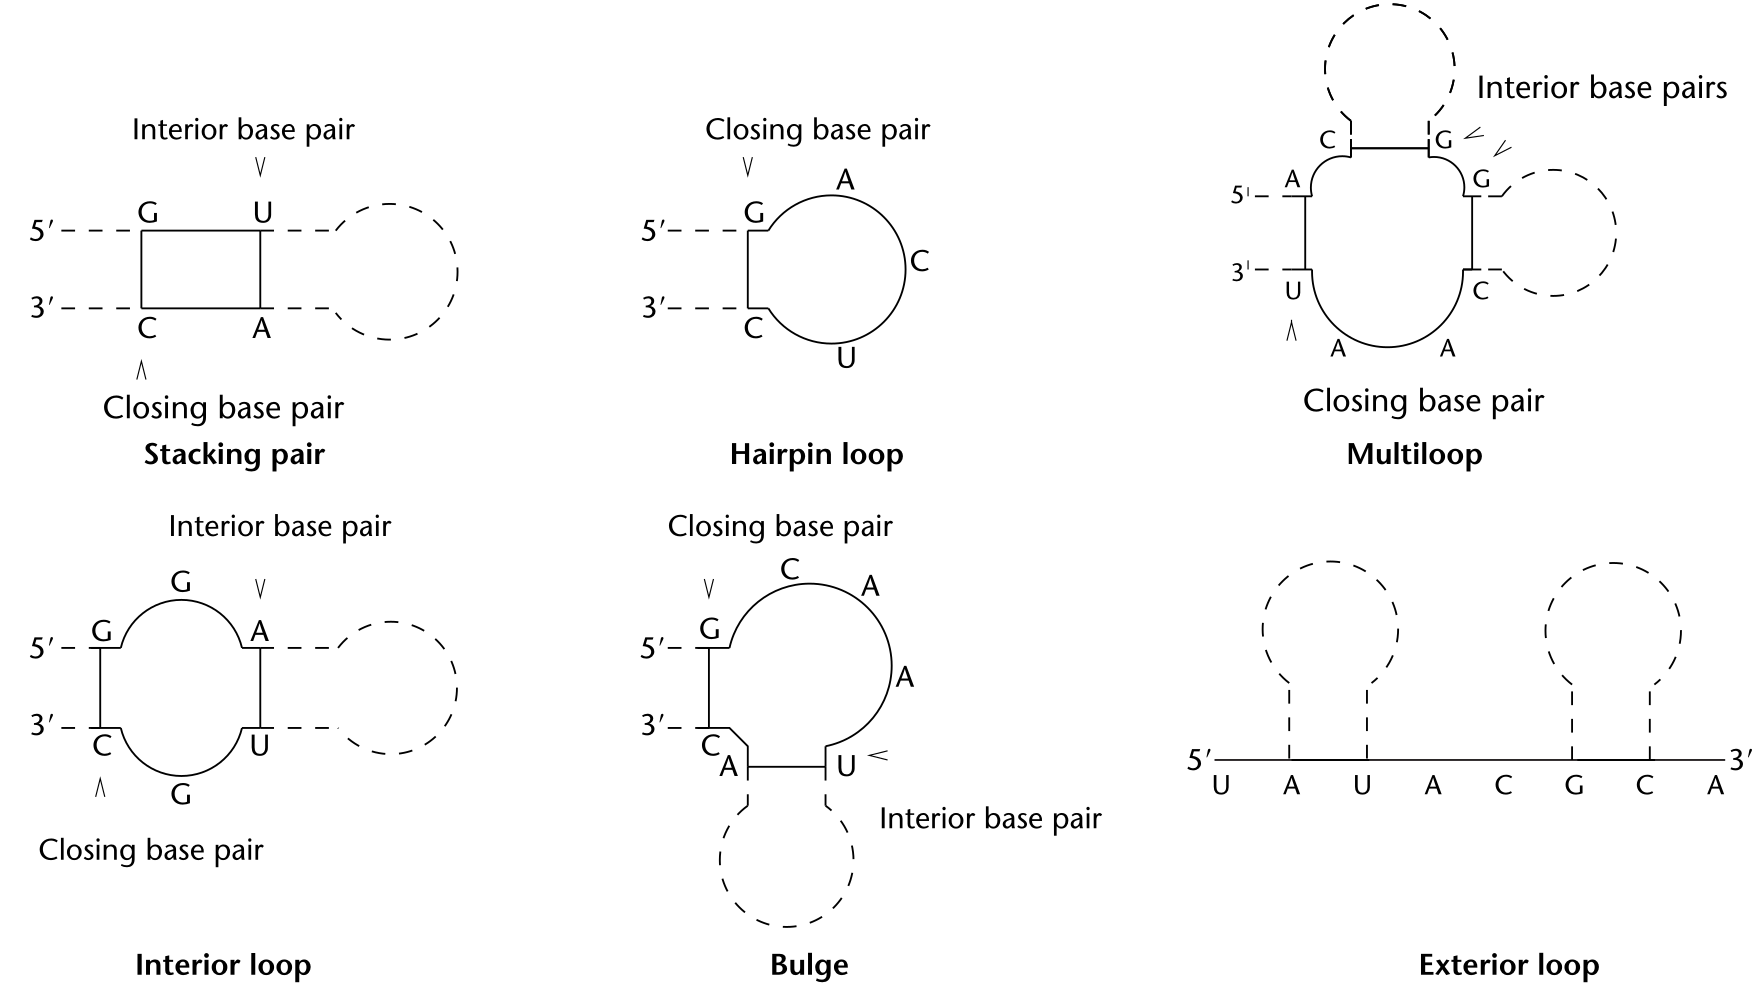
\includegraphics[width=0.9\textwidth]{pic/intro/notmine/hofacker2005_fig2mod.png}
	\caption[Loop Types]{Types of loops considered in a loop decomposition of RNA secondary structures.
		Essentially, only stacking pairs have stabilizing effects.
		The destabilizing energy contribution of loops largely depends on their symmetry and enclosed unpaired nucleotides.
		Per convention, the exterior loop, or open chain, serves as a reference point relative to which free energy changes are defined.
		Modified after \parencite[Figure 2]{hofacker_rna_2005}.
	}\label{fig:looptypes}
\end{figure}
\newpage
As a simplified example, the destabilizing free energy contribution $\Delta G_\mathrm{multi}$ of a multiloop as seen in \autoref{fig:looptypes} may be modelled as
\begin{equation}\label{eq:multi}
	\Delta G_\mathrm{multi} = \Delta G_\mathrm{init} + b \Delta G_\mathrm{branch} + u \Delta G_\mathrm{unpaired}
\end{equation}
where $b$ is the number of all surrounding base pairs and $u$ the number of base pairs \parencite{dirks_partition_2003}.

Over time, energy values for stacked base pairs and the different loop types have been measured experimentally and used to estimate secondary structures \parencite{tinoco_estimation_1971, tinoco_improved_1973}.
Continuous improvements on such energy estimations for loops and unusual substructures eventually lead to comprehensive sets of energy parameters widely used in thermodynamical structure prediction \parencite{turner_nndb_2010}.

Moreover, decomposition of a secondary structure into loops may be accomplished uniquely by identifying each loop with its closing base pair (see \autoref{fig:looptypes}) \parencite{hofacker_combinatorics_1998}.
These closing base pairs are defined based on the 5'$\rightarrow$3' direction of the sequence allowing to enumerate base pairs (and loops) in a precise order.
%It is easy to see that the base pairs of a secondary structure can be uniquely ordered by looking at a dot-bracket representation like in \autoref{fig:strucrepresentation:b} and ordering them according to the position of their opening parentheses.
Many structure prediction algorithms like the ones introduced in \autoref{ssub:theory:folding} build on this loop decomposition.
%\todo{more details on decomposition, bulges, in particular \unit[1]{nt} bulges}
%\subsubsection{Loop Decomposition}
%\label{ssub:intro:loops}

\end{document}
